%Hecho por Héctor Fernando Carrera Soto | hfcarrerasoto.usac@gmail.com

\documentclass[12pt,letterpaper]{exam}
\usepackage[left=1.5cm,right=1.5cm,top=1.5cm,bottom=1.8cm]{geometry}

\usepackage{dcolumn}% Align table columns on decimal point
\usepackage{bm}% bold math
%
%Paquete de Idioma
\usepackage[spanish]{babel}
%
%Codificación Alfabeto
\usepackage[utf8]{inputenc}
%
%Codificación de Fuente
\usepackage[T1]{fontenc}
%
%Índice
\usepackage{makeidx}
%
%Gráficos
\usepackage{graphicx}
\usepackage{subfig}
%\usepackage{xcolor} 
%
%Matemática
\usepackage{amsmath}
\usepackage{amsfonts}
\usepackage{amssymb}
%\usepackage{amstext} 
%
%Estilo de Página Numeración superior
%\pagestyle{headings}
%
%Hiperlinks \href{url}{text}
\usepackage[pdftex]{hyperref}
%
%Graficos y tablas
\usepackage{multirow}
%\usepackage{multicol}

%El paquete float es importante para las imágenes con la opción [H] para que las imágenes se coloquen en donde lo deseamos
\usepackage{float}
\usepackage{booktabs}
%
\decimalpoint
%\bibliographystyle{IEEEtran}
%\bibliography{IEEEabrv,mybibfile}
%Para tachar dimencionales
\usepackage{cancel}
%
%%<<<<<<<<<<<<<<<<<<<<  >>>>>>>>>>>>>>>>>>>
%<<<<<<<<<<<<<<<<<<<<  >>>>>>>>>>>>>>>>>>>
%<<<<<<<<<<<<<<<<<<<<  >>>>>>>>>>>>>>>>>>>
%	  Paquetes agregados al formato
%<<<<<<<<<<<<<<<<<<<<  >>>>>>>>>>>>>>>>>>>
%<<<<<<<<<<<<<<<<<<<<  >>>>>>>>>>>>>>>>>>>
%<<<<<<<<<<<<<<<<<<<<  >>>>>>>>>>>>>>>>>>>


%<<<<<<<<< Comando valores absolutos |x| >>>>>
\newcommand{\abs}[1]{\lvert1\rvert}
%<<<<<<<<< Comando para la normal ||x|| >>>>>
\newcommand{\norm}[1]{\lVert1\rVert}

%<<<<<<<<< para saltos de página usar  \clearpage >>>>>
%<<<<<<<<< para saltos entre líneas usar \vspace{2cm}>>>>>
%<<<<<<<<< para espaciado horizontal \hspace{1cm}>>>>>
%<<<<<<<<< para colocar url o referencias a url usar \url{http://www.latex-project.org/} o  \href{http://www.latex-project.org/}{latex project}>>>>>>>

%<<<<<<<<<<<<<<<<<<<<  >>>>>>>>>>>>>>>>>>>

%Paquete para configurar medidas de las tablas
\usepackage{tabularx}
%Forma del comando
%\begin{tabular}{|m{0.22\linewidth}|m{0.22\linewidth}|}


%<<<<<<<<< Para configurar \begin{enumerate}[A)]  en donde está la letra "A" escogemos como queremos enumerar, ejemplo \begin{enumerate}[i)]>>>>>>>>>>>>>>

\usepackage{enumerate}

%<<<<<<<<< Cambiar columnas >>>>>

%Se aconseja colocar el documento a una columna y luego cambiarle con forme se vaya utilizando. comandos:
%\begin{multicols}{2}
	%contenido
%\end{multicols}
\usepackage{multicol} %Paquete cambiar columnas

%<<<<<<<<<<<<<<<<<<<<  >>>>>>>>>>>>>>>>>>>

%Configurar sangría
\setlength{\parindent}{0pt}

%>>>>>>>>>>>>>>>>>>Esto es para interlineado V2<<<<<<<

%Para interlineado
%\renewcommand{\baselinestretch}{1.5}

%Para cambiar la sangría 2
%\setlength{\parindent}{4em}

%Espaciado entre parrafos
%\setlength{\parskip}{1em}

%Separación entre columnas
%Con una línea en medio
%\setlength\columnseprule{1pt}
%Sin una línea en medio
\setlength\columnsep{1cm}

%<<<<<<<<<<<<<<<<<<<<  >>>>>>>>>>>>>>>>>>>

%Para colocar punto decimal en lugar de coma automático.
\spanishdecimal{.}

%Para colocar anotaciónes al pié de página, podemos utilizar \footnote{Anotación pié de página}, pegado a la palabra a la cuál se hará la anotación.

%<<<<<<<<<<<<<<<<<<<<  >>>>>>>>>>>>>>>>>>>

%Para agregar un índice: \tableofcontents



%<<<<<<<<<<<<<<<<<<<<  >>>>>>>>>>>>>>>>>>>

% El comando \ balance se puede utilizar para equilibrar las columnas en la página final si se desea. Debe colocarse en cualquier lugar dentro de la primera columna de la última página.
\usepackage{balance}

%\balance
%<<<<<<<<<<<<<<<<<<<<  >>>>>>>>>>>>>>>>>>>

%Use el paquete pdfpages.
%Para incluir todas las páginas en el archivo PDF:
% \includepdf[pages=-]{myfile.pdf}

%Para incluir solo la primera página de un PDF:
%\includepdf[pages={1}]{myfile.pdf}

%Ejecute texdoc pdfpages en un Shell para ver el manual completo de pdfpages.

\usepackage{pdfpages}



%<<<<<<<<<<<<<<<<<<<<  >>>>>>>>>>>>>>>>>>>

%Este comando sirve para importar archivos txt.

\usepackage{verbatim}

% Usar \verbatiminput{archivo.tex}



%<<<<<<<<<<<<<<<<<<<<  >>>>>>>>>>>>>>>>>>>
%Para agregar una caratula más personalizada
%\begin{titlepage}
%	*
%\begin{titlepage}

%<<<<<<<<<<<<<<<<<<<<  >>>>>>>>>>>>>>>>>>>

%Para agregar texto entre ecuaciónes
%\textup{•}
%<<<<<<<<< Permite poner varios autores >>>>>>>>>>>>>

\usepackage{authblk}

%\author[1]{Author \thanks{correo1•university.edu}}
%\author[1]{Author \thanks{correo2•university.edu}}
%\author[1]{Author \thanks{correo3•university.edu}}
%\author[2]{Author \thanks{correo3•university.edu}}
%\author[2]{Author %\thanks{correo4•university.edu}}

%\affil[1]{Department of Computer Science, \LaTeX\ University}
%\affil[2]{Department of Mechanical Engineering, \LaTeX\ University}

%<<<<<<<<<<<<<<<<<<<<  >>>>>>>>>>>>>>>>>>>
%<<<<<<<<<<<<<<<<<<<<  >>>>>>>>>>>>>>>>>>>

\begin{document}

% Please add the following required packages to your document preamble:
% \usepackage{multirow}
\begin{title}

\begin{table}[]
\begin{tabular}{cllll}
\multirow{5}{*}{
\includegraphics[scale=1]{usac.png}} & Universidad de San Carlos de Guatemala.    &  & Sección:         & P1 \\
    & Facultad de ingeniería.                    &  &                  &            \\
    & EIME. 									 &  & Fecha de entrega:& 09/08/2022 \\
    & Química general.        &  &                  &            \\
    & Nombre: Héctor Fernando Carrera Soto.      &  & Carné:           & 201700923
\end{tabular}
\\
\begin{huge}
\begin{center}
\textbf{Calibración de material volumétrico}
\end{center}
\end{huge}

\end{table}

\end{title}

\header{Laboratorio química general - P1}{Héctor Fernando Carrera Soto}{201700923}
\headrule



%%%%%%%%%%%%%%%%%%%%%%%%%%%%%
%	Inicia el documento		%
%%%%%%%%%%%%%%%%%%%%%%%%%%%%%

\section{Calibración de una pipeta}

\subsection{Datos de la pipeta y clasificación de los instrumentos}



\begin{multicols}{2}

\subsubsection*{Intrumentos TD\footnote{To delivery o para verter.}}

%%%

\begin{figure}[H]
\centering
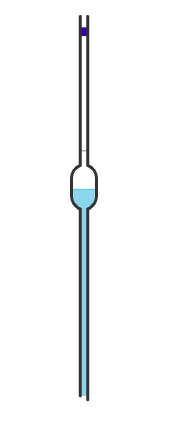
\includegraphics[scale=0.4]{pipeta.png}
\caption{Pipeta.}
\begin{center}
Fuente: Elaboración propia.
\end{center}
\label{fig:pipeta}
\end{figure}


\paragraph{Pipeta volumétrica:} No tiene las puntas graduadas y solo mide un volumen.

\paragraph{Volumen nominal de la pipeta de la figura \ref{fig:pipeta}:} $25 \ mL$

%%%

\subsubsection*{Intrumentos TC\footnote{To contain o para contener.}}

\begin{figure}[H]
\centering
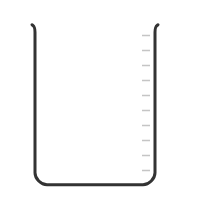
\includegraphics[scale=0.5]{Beaker.png}
\caption{Beaker.}
\begin{center}
Fuente: Elaboración propia.
\end{center}
\label{fig:Beaker}
\end{figure}

%%%

\subsubsection*{Intrumentos complementarios}

\begin{figure}[H]
\centering

\includegraphics[scale=0.5]{1-proce_5.png}
\caption{Termómetro digital.}
\begin{center}
Fuente: Elaboración propia.
\end{center}
\label{fig:Termómetro}
\end{figure}


\begin{figure}[H]
\centering
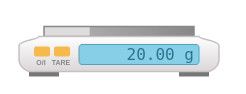
\includegraphics[scale=0.5]{Balanza.png}
\caption{Balanza.}
\begin{center}
Fuente: Elaboración propia.
\end{center}
\label{fig:Balanza}
\end{figure}


\begin{figure}[H]
\centering
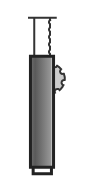
\includegraphics[scale=0.5]{Pipeteador.png}
\caption{Pipeteador.}
\begin{center}
Fuente: Elaboración propia.
\end{center}
\label{fig:Pipeteador}
\end{figure}


%%%

\end{multicols}

%%%%%%%%%%%%%%
%\clearpage
\subsection{Procedimiento}

%
\includegraphics[scale=0.5]{identificación.png} 


\begin{multicols}{2}

Se llenó la pipeta hasta la marca de aforo, sabiendo que su volumen nominal es de $25 \ mL$.


\begin{figure}[H]
\centering
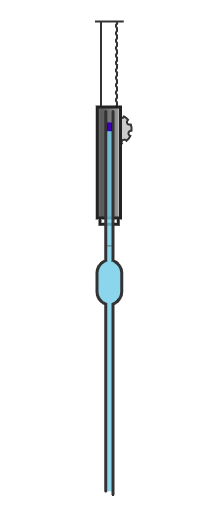
\includegraphics[scale=0.4]{1-proce_1.png}
\caption{Elaboración propia.}
\label{fig:1-proce_1}
\end{figure}

Se vació lentamente tocando la punta de la pipeta la pared interna del beaker, se repitió tres veces más con la misma pipeta y los otros beakers.

\begin{figure}[H]
\centering
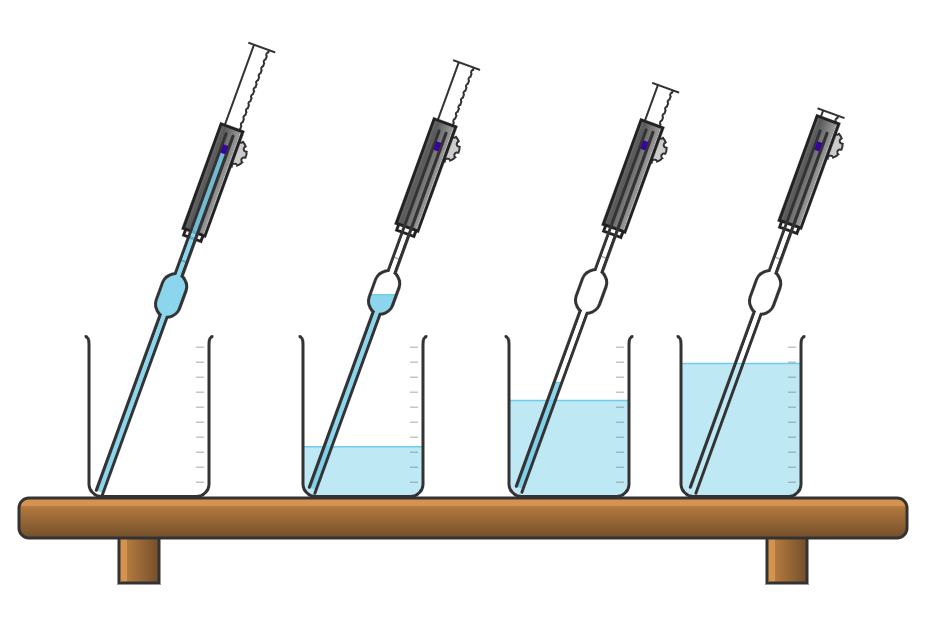
\includegraphics[width = \columnwidth]{1-proce_2.png}
\caption{Elaboración propia.}
\label{fig:1-proce_2}
\end{figure}

Se procedió a taparlos una vez llenados con la pipeta.

\begin{figure}[H]
\centering
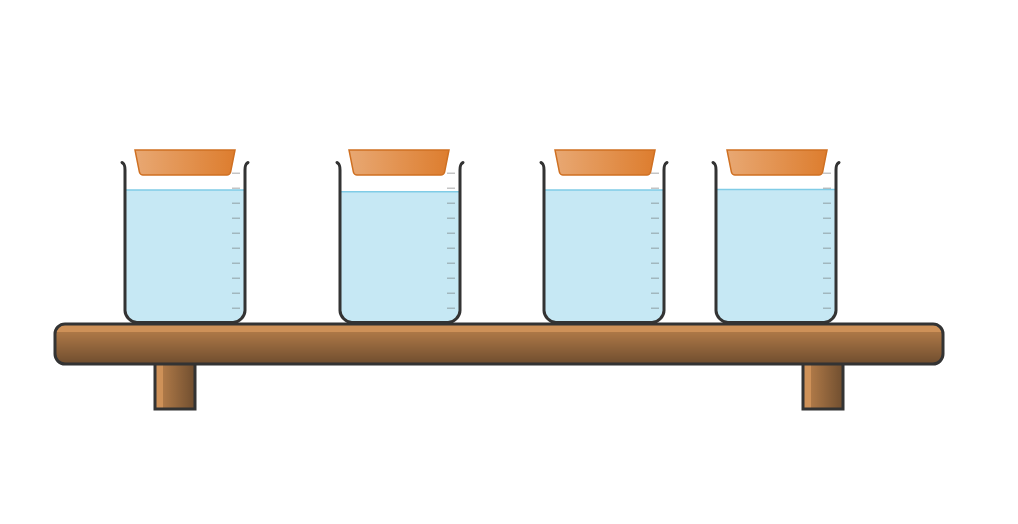
\includegraphics[width = \columnwidth]{1-proce_3.png}
\caption{Elaboración propia.}
\label{fig:1-proce_3}
\end{figure}

Se pesó cada beaker en una balanza digital.

\begin{figure}[H]
\centering
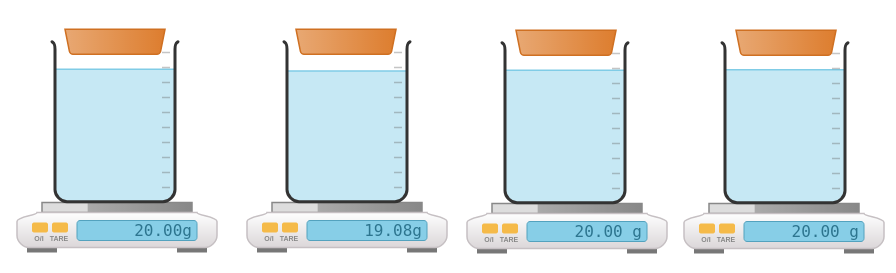
\includegraphics[width = \columnwidth]{1-proce_4.png}
\caption{Elaboración propia.}
\label{fig:1-proce_4}
\end{figure}

En la antigüedad, el agua era usado como punto de referencia en algunas medidas, ya que es una sustancia común en la naturaleza, por lo cual se usó como punto de referencia para el gramo, como se puede percatar en la figura \ref{fig:1-proce_4}, $20 \ mL$ de agua equivale a $20 \ g$ de agua.\\

Se procedió a medir la temperatura de agua siendo de $20^{\circ}C$ para cada beaker.

\begin{figure}[H]
\centering

\includegraphics[scale=0.5]{1-proce_5.png}
\caption{Elaboración propia.}
\label{fig:1-proce_5}
\end{figure}

\end{multicols}






%%%%%%%%%%%%%%%%%%%%%%%%%%%%%
%%%%%%%%%%%%%%%%%%%%%%%%%%%%%

\section{Calibración de un balón aforado}

\subsection{Datos del balón aforado y clasificación de los instrumentos}

\begin{multicols}{2}

\subsubsection*{Intrumentos TD}

%%%

\begin{figure}[H]
\centering
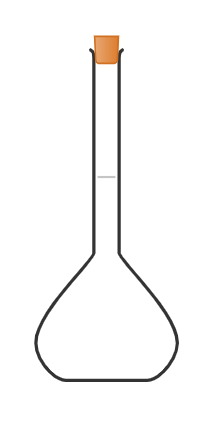
\includegraphics[scale=0.5]{2-1.png}
\caption{Balón aforado.}
\begin{center}
Fuente: Elaboración propia.
\end{center}
\label{fig:balón_con_tapa-2}
\end{figure}

\paragraph{Volumen nominal del balón aforado de la figura \ref{fig:balón_con_tapa-2}:} $25 \ mL$

%%%

\subsubsection*{Intrumentos TC}

\begin{figure}[H]
\centering
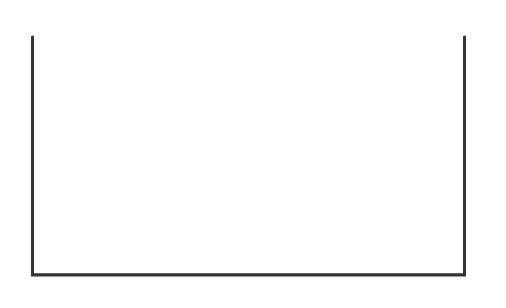
\includegraphics[width = \columnwidth]{2-6.png}
\caption{Contenedor de líquido.}
\begin{center}
Fuente: Elaboración propia.
\end{center}
\label{fig:Tanque-2}
\end{figure}

%%%

\subsubsection*{Intrumentos complementarios}

\begin{figure}[H]
\centering

\includegraphics[scale=0.5]{1-proce_5.png}
\caption{Termómetro digital.}
\begin{center}
Fuente: Elaboración propia.
\end{center}
\label{fig:Termómetro}
\end{figure}


\begin{figure}[H]
\centering
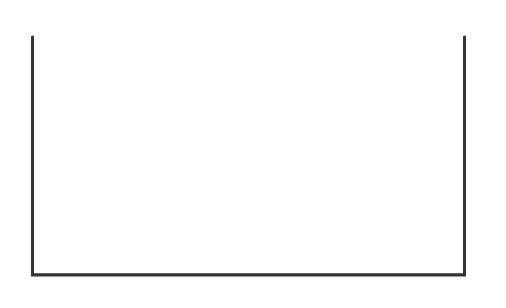
\includegraphics[width = \columnwidth]{2-6.png}
\caption{Contenedor de agua.}
\begin{center}
Fuente: Elaboración propia.
\end{center}
\label{fig:2-Contenedor}
\end{figure}

%%%

\end{multicols}

%%%%%%%%%%%%%%
%\clearpage
\subsection{Procedimiento}


\begin{multicols}{2}

\subsubsection{Primera corrida}

Antes de cada corrida, se taró el balón aforado, como se muestra en la figura \ref{fig:2-tara}.

\begin{figure}[H]
\centering
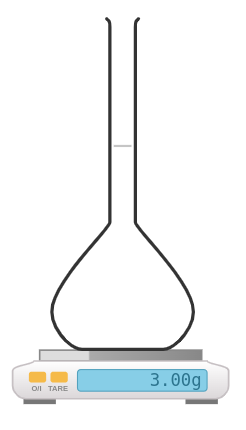
\includegraphics[scale=0.4]{Balón_tarado.png}
\caption{Tara del balón aforado.}
\begin{center}
Fuente: Elaboración propia.
\end{center}
\label{fig:2-tara}
\end{figure}

Se llenó hasta la marca, en la parte inferior del menisco de forma tangencial del balón aforado, como se muestra en la figura \ref{fig:2-balón_1}, \ref{fig:2-balón_2} y \ref{fig:2-balón_3}.

\begin{figure}[H]
\centering
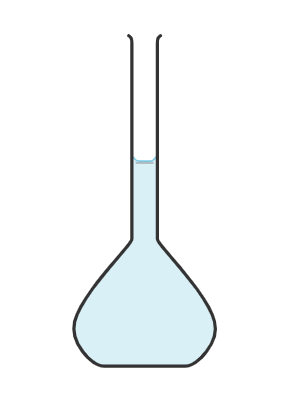
\includegraphics[scale=0.4]{2-2.png}
\caption{Llenado de la primera corrida.}
\begin{center}
Fuente: Elaboración propia.
\end{center}
\label{fig:2-balón_1}
\end{figure}

Se pesó la masa del balón aforado lleno, como se muestran en la figura \ref{fig:2-Peso_1}, \ref{fig:2-Peso_2} y \ref{fig:2-Peso_3}.


\begin{figure}[H]
\centering
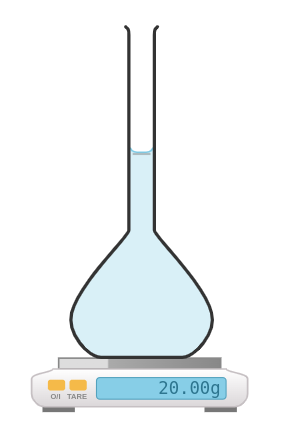
\includegraphics[scale=0.4]{2-8.png}
\caption{Peso de la primera corrida de la figura \ref{fig:2-balón_1}.}
\begin{center}
Fuente: Elaboración propia.
\end{center}
\label{fig:2-Peso_1}
\end{figure}

Se vació el balón en cada corrida y se repitió el proceso con el mismo balón aforado como se muestra en las figuras \ref{fig:2-vaciado_1}, \ref{fig:2-vaciado_2} y \ref{fig:2-vaciado_3}.

\begin{figure}[H]
\centering
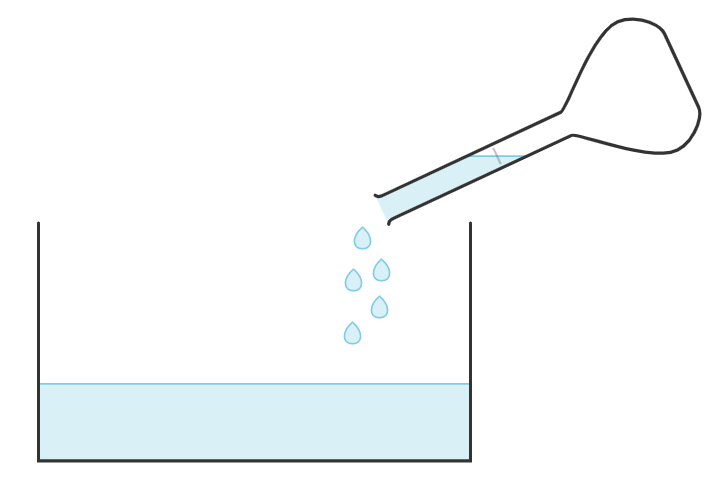
\includegraphics[width = \columnwidth]{2-5.png}
\caption{Vaciado de la primera corrida de la figura \ref{fig:2-balón_1}.}
\begin{center}
Fuente: Elaboración propia.
\end{center}
\label{fig:2-vaciado_1}
\end{figure}

Se tomó la temperatura del lugar, figura \ref{fig:2-Termómetro_1}, \ref{fig:2-Termómetro_2} y \ref{fig:2-Termómetro_3}.

\begin{figure}[H]
\centering

\includegraphics[scale=0.5]{1-proce_5.png}
\caption{Medición de temperatura con termómetro digital de la primera corrida de la figura \ref{fig:2-balón_1}.}
\begin{center}
Fuente: Elaboración propia.
\end{center}
\label{fig:2-Termómetro_1}
\end{figure}


%%%%%%%%%%%%%%

\subsubsection{Segunda corrida}

\begin{figure}[H]
\centering
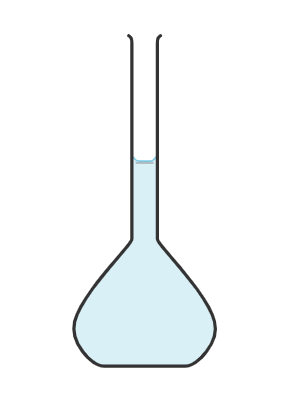
\includegraphics[scale=0.4]{2-2.png}
\caption{Llenado de la segunda corrida.}
\begin{center}
Fuente: Elaboración propia.
\end{center}
\label{fig:2-balón_2}
\end{figure}

\begin{figure}[H]
\centering
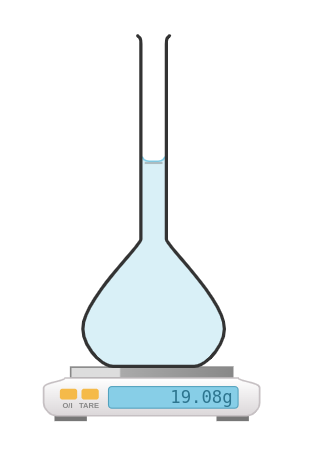
\includegraphics[scale=0.4]{2-7.png}
\caption{Peso de la primera corrida de la figura \ref{fig:2-balón_2}.}
\begin{center}
Fuente: Elaboración propia.
\end{center}
\label{fig:2-Peso_2}
\end{figure}


\begin{figure}[H]
\centering
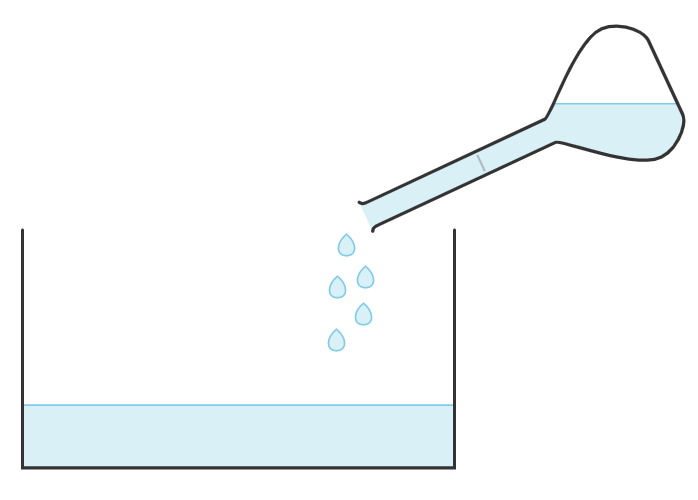
\includegraphics[width = \columnwidth]{2-4.png}
\caption{Vaciado de la segunda corrida de la figura \ref{fig:2-balón_2}.}
\begin{center}
Fuente: Elaboración propia.
\end{center}
\label{fig:2-vaciado_2}
\end{figure}


\begin{figure}[H]
\centering

\includegraphics[scale=0.5]{1-proce_5.png}
\caption{Medición de temperatura con termómetro digital de la primera corrida de la figura \ref{fig:2-balón_2}.}
\begin{center}
Fuente: Elaboración propia.
\end{center}
\label{fig:2-Termómetro_2}
\end{figure}

%%%%%%%%%%%%%%

\subsubsection{Tercera corrida}

\begin{figure}[H]
\centering
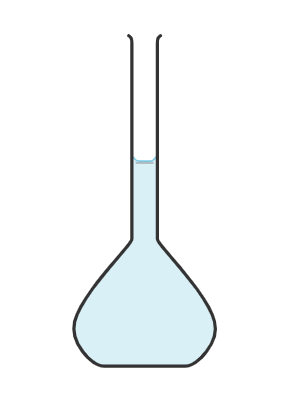
\includegraphics[scale=0.4]{2-2.png}
\caption{Llenado de la tercera corrida.}
\begin{center}
Fuente: Elaboración propia.
\end{center}
\label{fig:2-balón_3}
\end{figure}


\begin{figure}[H]
\centering
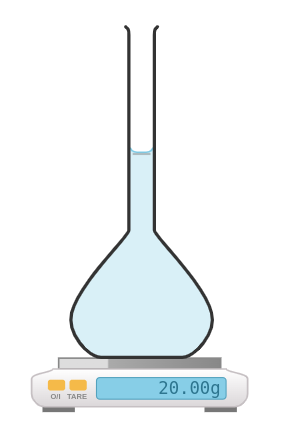
\includegraphics[scale=0.4]{2-8.png}
\caption{Peso de la primera corrida de la figura \ref{fig:2-balón_3}.}
\begin{center}
Fuente: Elaboración propia.
\end{center}
\label{fig:2-Peso_3}
\end{figure}


\begin{figure}[H]
\centering
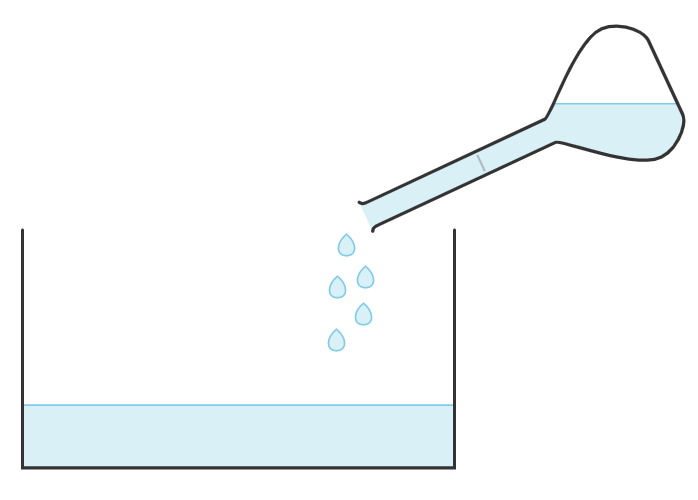
\includegraphics[width = \columnwidth]{2-4.png}
\caption{Vaciado de la tercera corrida de la figura \ref{fig:2-balón_3}.}
\begin{center}
Fuente: Elaboración propia.
\end{center}
\label{fig:2-vaciado_3}
\end{figure}


\begin{figure}[H]
\centering

\includegraphics[scale=0.5]{1-proce_5.png}
\caption{Medición de temperatura con termómetro digital de la primera corrida de la figura \ref{fig:2-balón_3}.}
\begin{center}
Fuente: Elaboración propia.
\end{center}
\label{fig:2-Termómetro_3}
\end{figure}


\end{multicols}

%%%%%%%%%%%%%%%%%%%%%%%%%%%%%
%%%%%%%%%%%%%%%%%%%%%%%%%%%%%

\clearpage

\section{Señales de riesgo y prevención}

\begin{multicols}{2}

\begin{figure}[H]
\centering
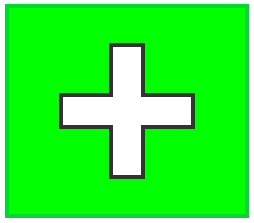
\includegraphics[width = \columnwidth]{Señal-2.png}
\caption{Primeros auxilios.}
\begin{center}
Fuente: Elaboración propia.
\end{center}
\label{fig:Señal_1}
\end{figure}


\begin{figure}[H]
\centering

\includegraphics[width = \columnwidth]{Señal-1.png}
\caption{Uso de mascarilla en la campana de extracción.}
\begin{center}
Fuente: Elaboración propia.
\end{center}
\label{fig:Señal_2}
\end{figure}

\end{multicols}

%\balance
\end{document}